\documentclass{article}
\usepackage{graphicx} % Required for inserting images
\usepackage[margin=1in]{geometry}
\usepackage{url}
\usepackage{hyperref}

\usepackage{float}
\usepackage{amsmath}


\title{CS310 Progress Report: Evaluating the Performance of Blink Detection on DeepFakes Injected With Adversarial Noise}
\author{Joel Coulon, 2204489}
\date{}

\begin{document}

\maketitle

\section{Project Introduction}

A DeepFake refers a video of an individual is digitally altered or created by an Artificial Intelligence (AI). These are often generated using Generative Adversarial Network (GANs) models and are trained via the adversarial of two models: one attempting to generate a realistic image, the other attempting to detect the inaccuracies. These two then train each other until the original model can generate videos that are deemed realistic by the detector.\\

Initially, these models were fairly obvious to detect, even for humans\ref{fig:earlyexample}. Various features, such as temporal inconsistencies, feature irregularities, and inconsistencies in lighting produced by GANs were all tell-tale signs of DeepFaked imagery. However, over time, GANs have developed resulting in DeepFakes now being almost impossible to tell apart from genuine videos by humans.

\begin{figure}[H]
    \centering
    \fbox{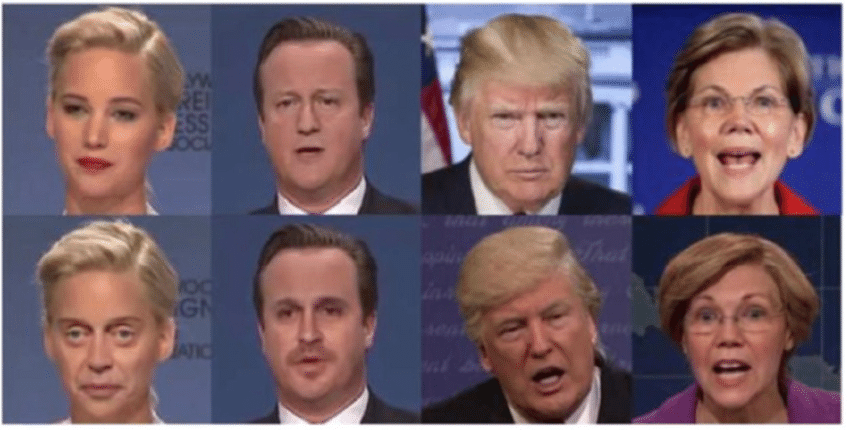
\includegraphics[width=0.5\linewidth]{images/Examples-of-original-and-deepfake-videos.png}}
    \caption{An early of example of DeepFakes with original images on the top, faked images on the bottom\cite{earlydeepfakeimage}}
    \label{fig:earlyexample}
\end{figure}

Due to their difficulty to be accurately identified by humans, DeepFakes soon became a popular way to spread misinformation by faking an individual's likeness. For example, DeepFakes were used by a variety of sources to promote political parties in the 2021 Lebanese elections\cite{misinformation}. The other primary use of DeepFakes is pornography with an estimated 98\% of DeepFakes being porn\cite{pornography}, including the first main-stream DeepFake in 2017 of actress Gal Gadot\cite{misinformation}.\\

Ever since the creation of DeepFakes there has been efforts to detect them. Original DeepFake detection methods relied on pixel analysis and visual artifacts present in early DeepFakes\cite{yu2021survey}. However through a combination of improvement in generation techniques and adversarial noise attacks\cite{huang2020fakeretouch}\cite{pertubations}, these original methods are proving increasingly ineffective.\\

One method proposed to tackle modern DeepFakes is blink detection. Blinking is a subconscious act for humans and falls into a predictable patterns. DeepFakes are notoriously bad at simulating blinking, either by not blinking at all or blinking in unnatural intervals. Thus methods have been used to leverage these temporal inconsistencies to detect DeepFakes with a high degree of accuracy\cite{blinking-pattern}.\\

So far, the resilience of blink-detection to adversarial noise has not been studied. It seems likely that due to this method relying on identification of features rather than individual pixels, it seems likely that adversarial noise would not affect the detection of a DeepFake in any meaningful way. This project aims to verify whether this assumption is true or not.

\section{Literature Review}

This project combines two thoroughly-research topics (Blink-based DeepFake detection and Adversarial noise injection) which have had extensive research on both of them.

\subsection{Blink Detection}
\subsubsection{DeepVision}

DeepVision\cite{blinking-pattern} is a model that takes into account the time, activity, gender and age of the individual in a video to determine whether a video is DeepFaked or not by comparing their blink patterns to a database of known ``good" blink frequencies\\

The pre-process stage of the model involves categorising the video based on 4 landmarks. The landmarks are: gender, age (in 6 sub-categories varying from \textless 20 to 65+), activity (dynamic or static), and time (am/pm). The frequency of a human varies based on all these features\cite{varying-blink}, and therefore they believe all of these factors need to be taken into account for an accurate detection.\\

To actually detect a blink, two algorithms are used. The first is an algorithm called Fast-HyperFace\cite{ranjan2017hyperface} which is used to detect the landmarks of the face, pose, and gender of the individual in a video. The key landmarks from this are then extracted to then aid in the performance of the second model: Eye-Aspect Ration (EAR). EAR uses 6 points to calculate the absolute area of the horizontal versus the vertical axis to determine if a blink has occurred\cite{EAR}.
\begin{equation}
    EAR=\frac{||p_2-p_6||+||p_3-p_5||}{2||p_1-p_4||}
\end{equation}
The average of the left eye ($EAR_l$) and the right ($EAR_r$) can then be taken to get the mean eye ration ($EAR_i$)
\begin{equation}
    EAR_i = \frac{EAR_l + EAR_r}{2}
\end{equation}
\begin{figure}[H]
    \centering
    \fbox{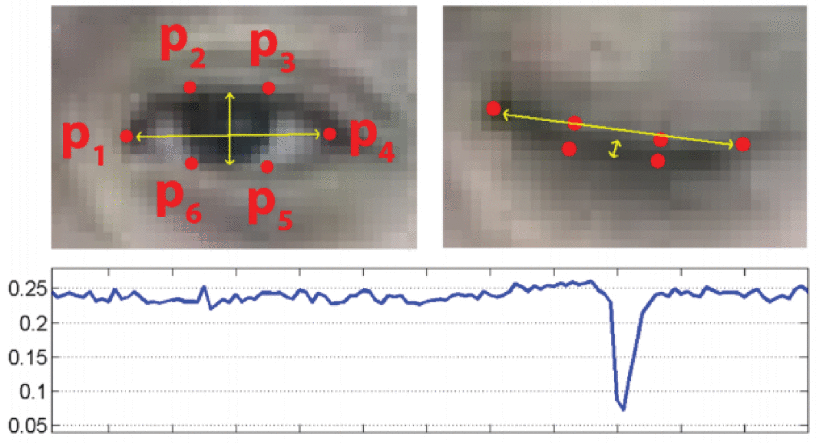
\includegraphics[width=0.5\linewidth]{images/EAR.png}}
    \caption{The EAR algorithm at work with eye landmarks $p_{1-6}$ labelled and a graph representing EAR (y-axis) over time (x-axis)}
    \label{fig:EAR}
\end{figure}

A blink is defined as when $EAR_i$ drops below a certain threshold for multiple consecutive frames. Data such as when the blink occurred in time, the period of blink, and frequency are all extracted and fed into the next stage.\\

This data is then compared with data from a pre-existing database of valid blinks derived from the Eye Blinking Prediction dataset from Kaggle\cite{eyeblinkprediction}. The factors mentioned above are all compared to see how similar they are to valid blinks in authentic videos and if it is within a certain threshold the video is deemed real. The paper does not mention this threshold. \\

DeepVision achieves an overall accuracy of 87.5\%\cite{blinking-pattern}.

\subsection{Adversarial Noise}
\subsection{Datasets}
\subsection{Noise Reduction}

\section{Current Progress}

\section{Future Progress}

\section{Appraisals \& Reflections}

\section{Legal, Social, Ethical, and Professional Issues \& Considerations}

\section{Project Management}

\bibliographystyle{IEEEtran}
\bibliography{progress}

\end{document}